\documentclass[a4paper,10pt,uplatex,dvipdfmx]{jsarticle}


% 数式
\usepackage{amsmath,amsfonts}
\usepackage{bm}
% 画像
\usepackage[dvipdfmx]{graphicx}
\usepackage{here}
% program
\usepackage{color}
\usepackage{listings, jlisting}
\input{listings-glsl.prf}
% 枠付き
\usepackage{ascmac}

\lstset{
 language={C++},%言語の指定
%  backgroundcolor={\color[gray]{.85}},%背景色と透過度
 basicstyle={\ttfamily},%書体の指定
 identifierstyle={\small\color[rgb]{0.8,0.5,0}},%キーワードでない文字の書体
 commentstyle={\small\itshape\color[rgb]{0,0.3,0}},%注釈の書体
 keywordstyle={\small\bfseries\color[rgb]{0,0.5,1}},%キーワード(int, ifなど)の書体指定
 ndkeywordstyle={\small},%
 stringstyle={\small\ttfamily\color[rgb]{1,0.5,0}},%文字列
 frame={tb},%枠縁(leftline,topline,bottomline,lines,trBL,shadowbox, single)
 breaklines=true,%折り返し(自動改行)
 breakindent = 10pt,  %自動改行後のインデント量(デフォルトでは20[pt])	
 columns=[l]{fullflexible},%
 numbers=left,%行番号表示
 xrightmargin=0zw,%
 xleftmargin=3zw,%
 numberstyle={\scriptsize},%行番号の書体指定
 stepnumber=1,
 numbersep=1zw,%
 lineskip=-0.5ex%
}
\renewcommand{\lstlistingname}{Code} % キャプション名の指定

\begin{document}
\title{アドバンストCG\\ \huge 第4回レポート}
\author{学籍番号:201811411\\ 所属:情報学群情報メディア創成学類\\ 氏名:加藤虎之介}
\date{\today}
\maketitle

\section{実行環境}
\subsection{実行に用いたOS}
macOS Big Sur ver11.3.1

\subsection{プログラム起動時に表示される情報}
\begin{screen}
  OpenGL version: 2.1 ATI-4.4.17\\
  GLSL version: 1.20\\
  Vendor: ATI Technologies Inc.\\
  Renderer: AMD Radeon Pro 5300M OpenGL Engine
\end{screen}

\section{課題A}
\subsection{修正したソースコード}
\lstinputlisting[caption = LoopSubdivision.cpp]{/Users/toranosuke/GoogleDrive/LectureDocument/2021/01_SpringSemester/AdvancedCG/code/day04/src/LoopSubdivision.cpp}
\lstinputlisting[caption = CatmullClarkSubdivision.cpp]{/Users/toranosuke/GoogleDrive/LectureDocument/2021/01_SpringSemester/AdvancedCG/code/day04/src/CatmullClarkSubdivision.cpp}

\subsection{実行結果}
\subsubsection{Loop細分割}
Loop細分割をcube.objに対して実行した結果は以下のようになった。
\begin{figure}[htbp]
  \begin{minipage}{0.33\hsize}
    \begin{center}
      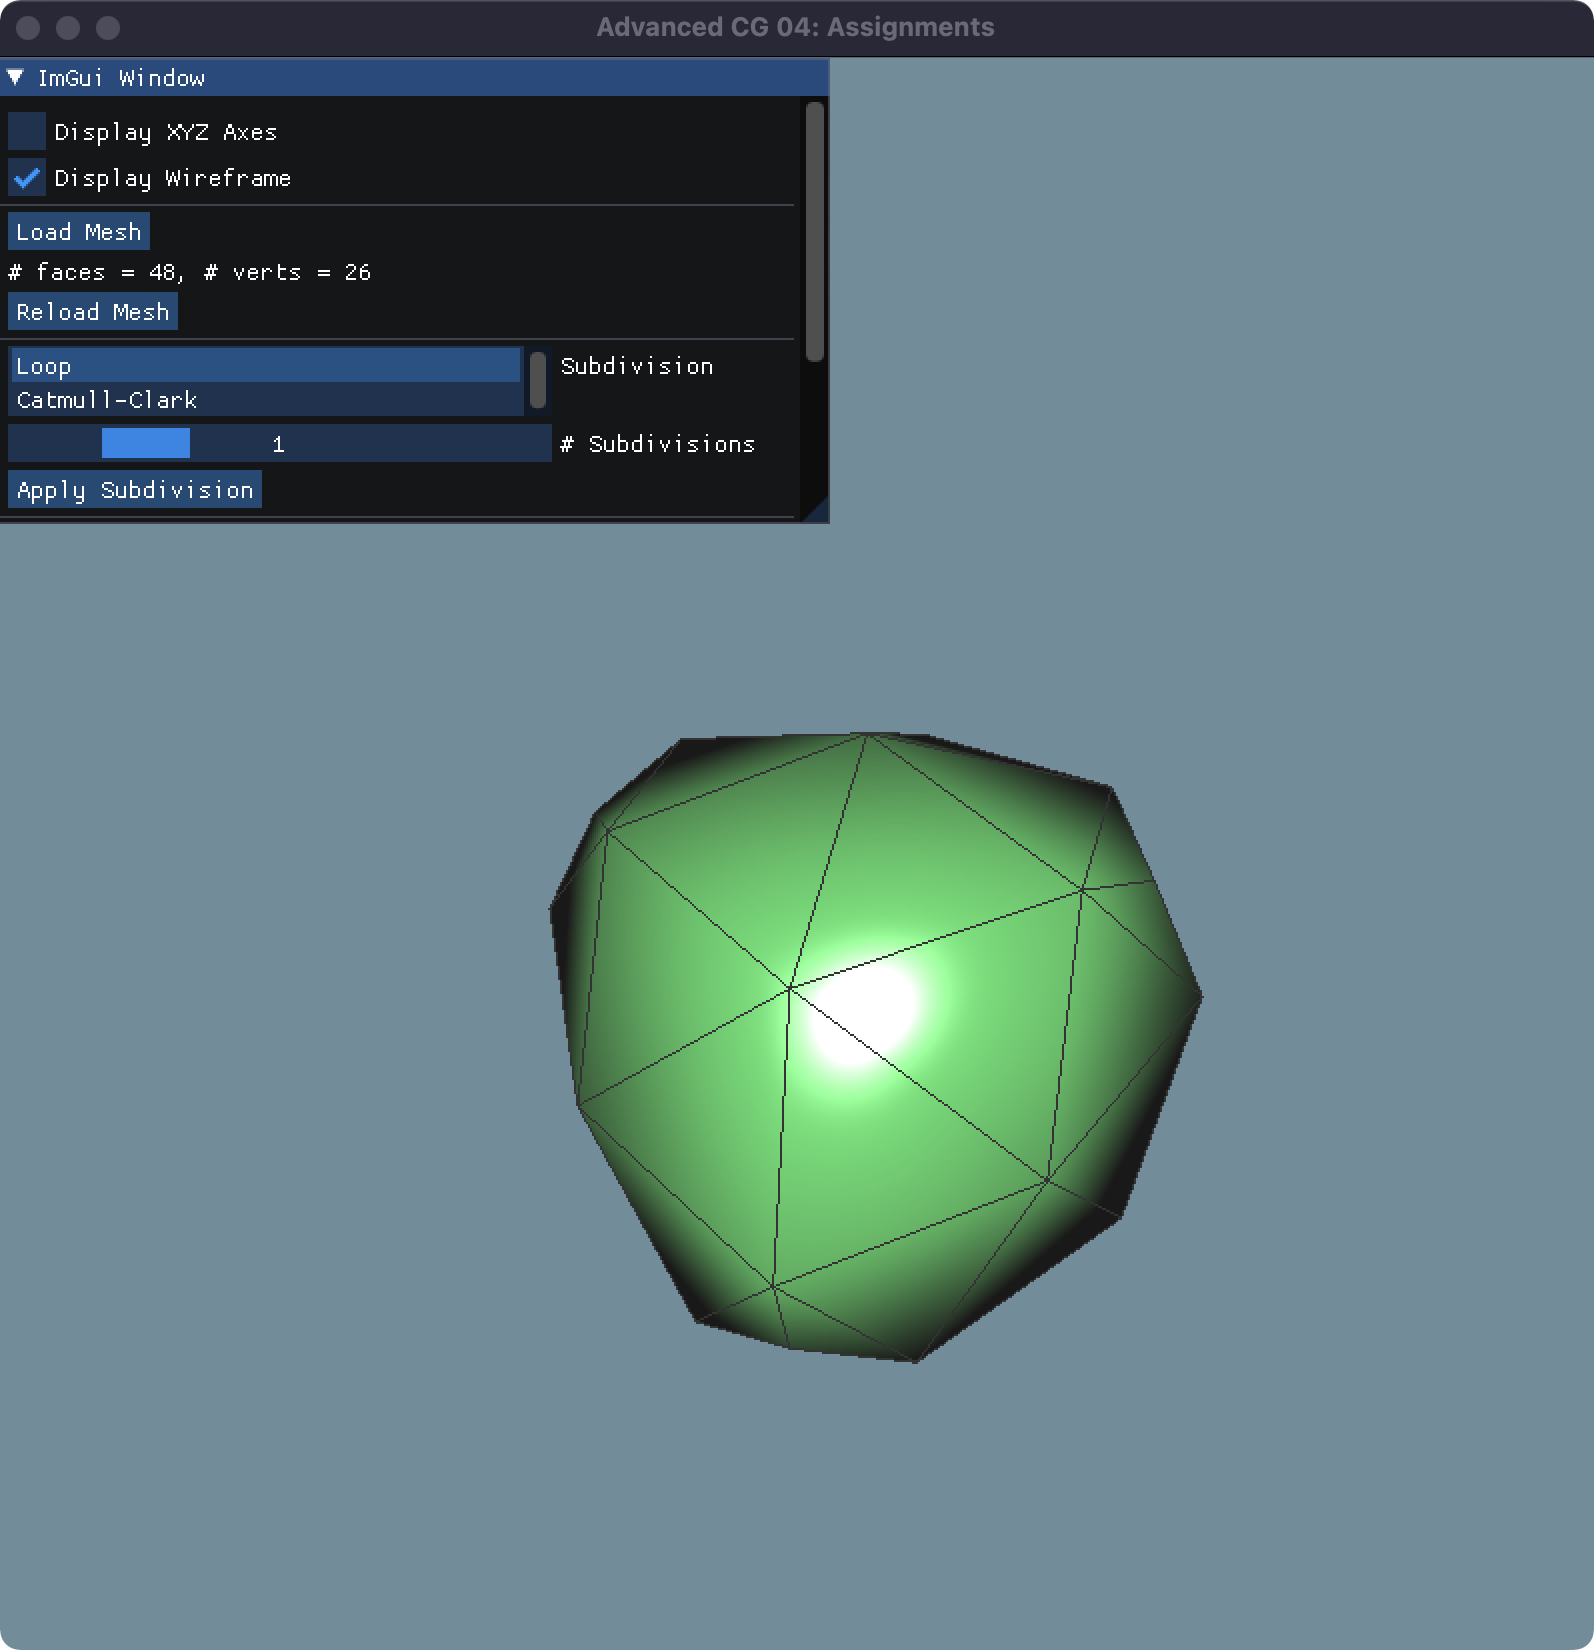
\includegraphics[width=45mm]{img/loop-cube-1.png}
      \caption{適用回数:1回}
    \end{center}
  \end{minipage}
  \begin{minipage}{0.33\hsize}
    \begin{center}
      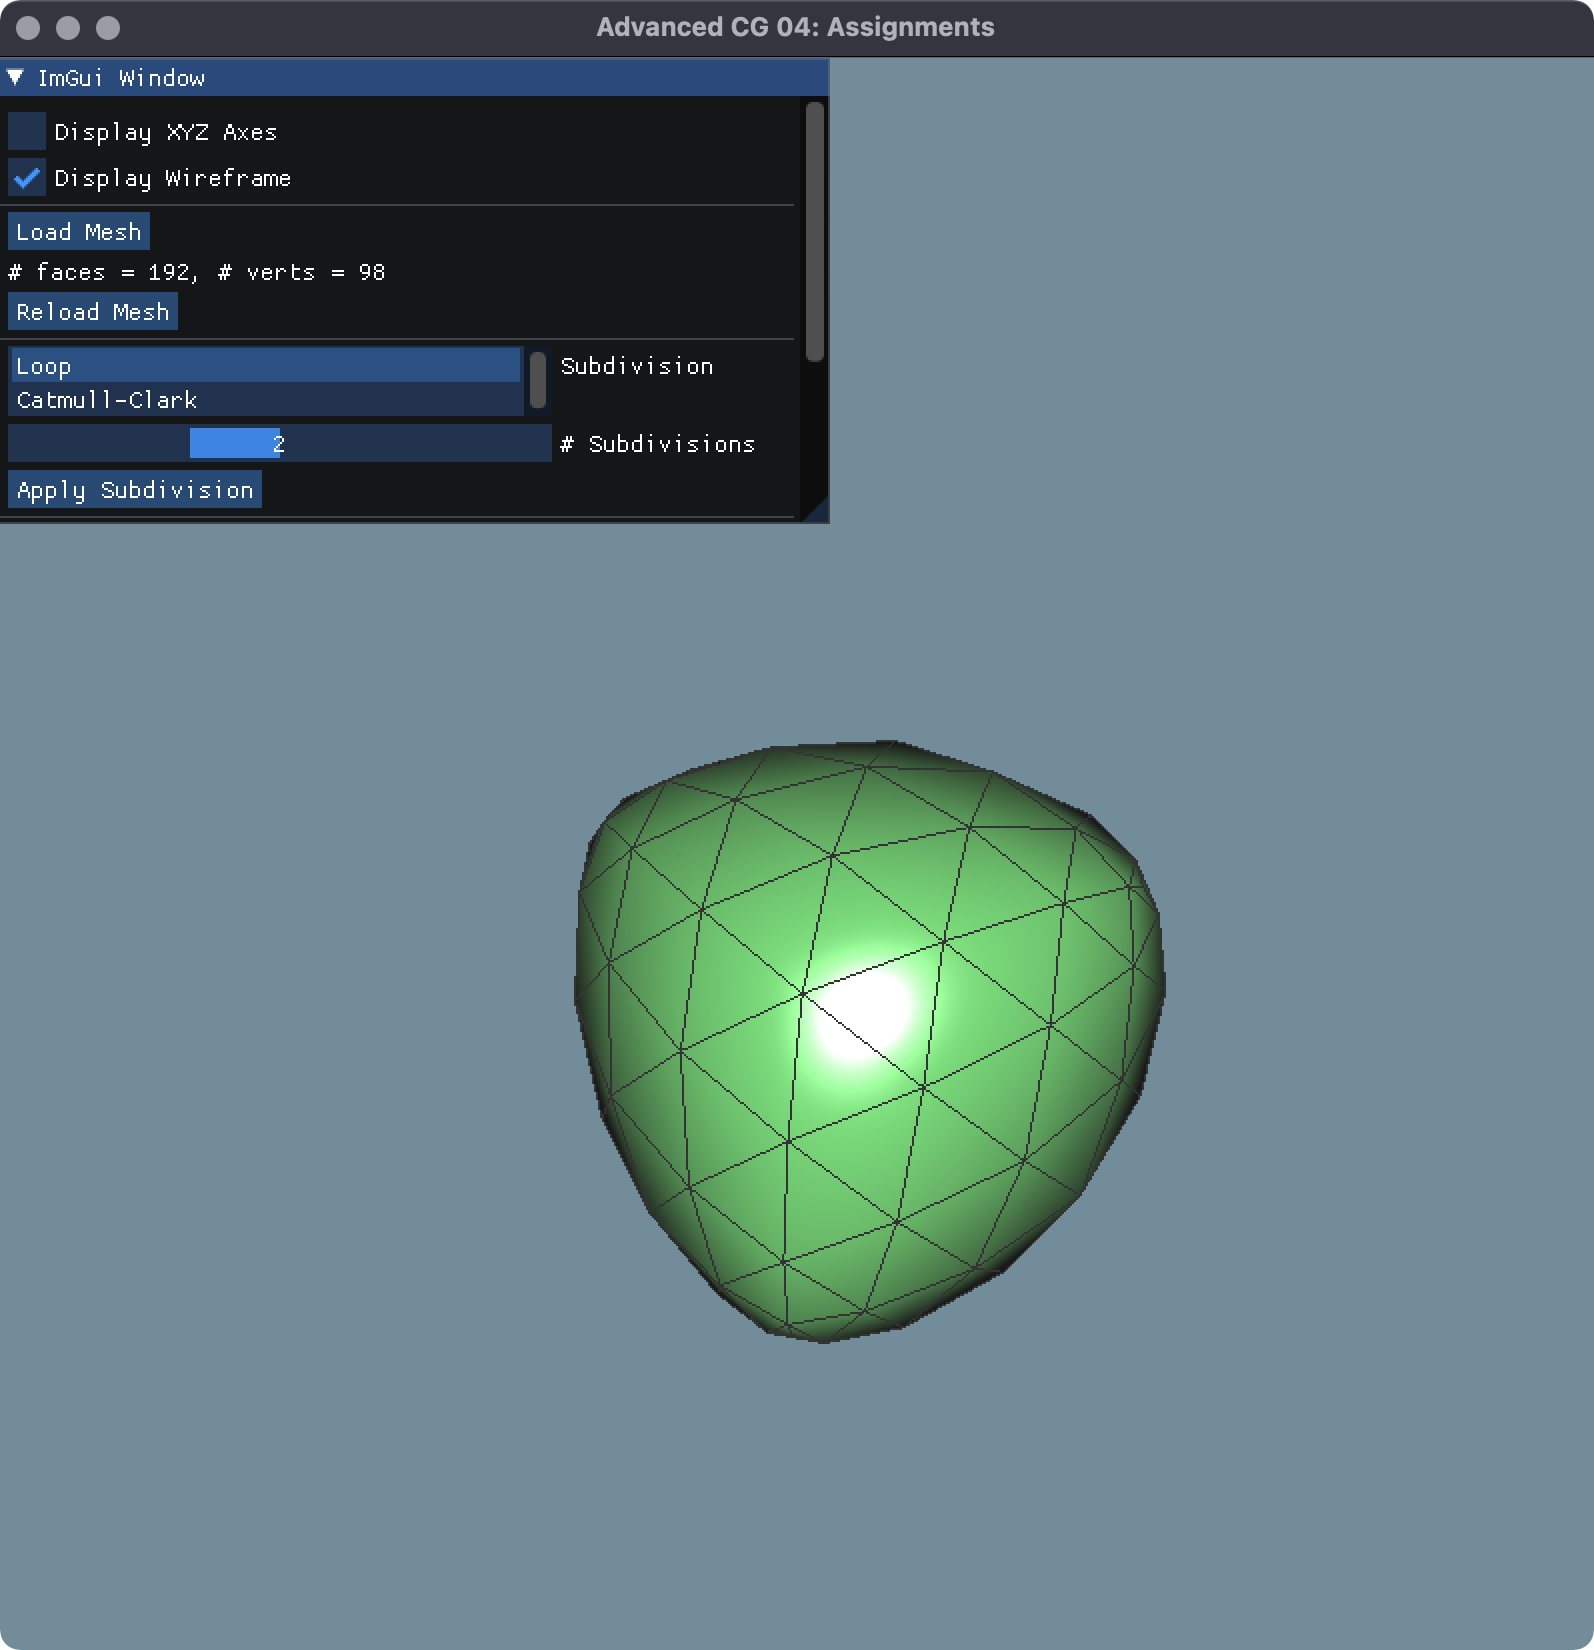
\includegraphics[width=45mm]{img/loop-cube-2.png}
      \caption{適用回数:2回}
    \end{center}
  \end{minipage}
  \begin{minipage}{0.33\hsize}
    \begin{center}
      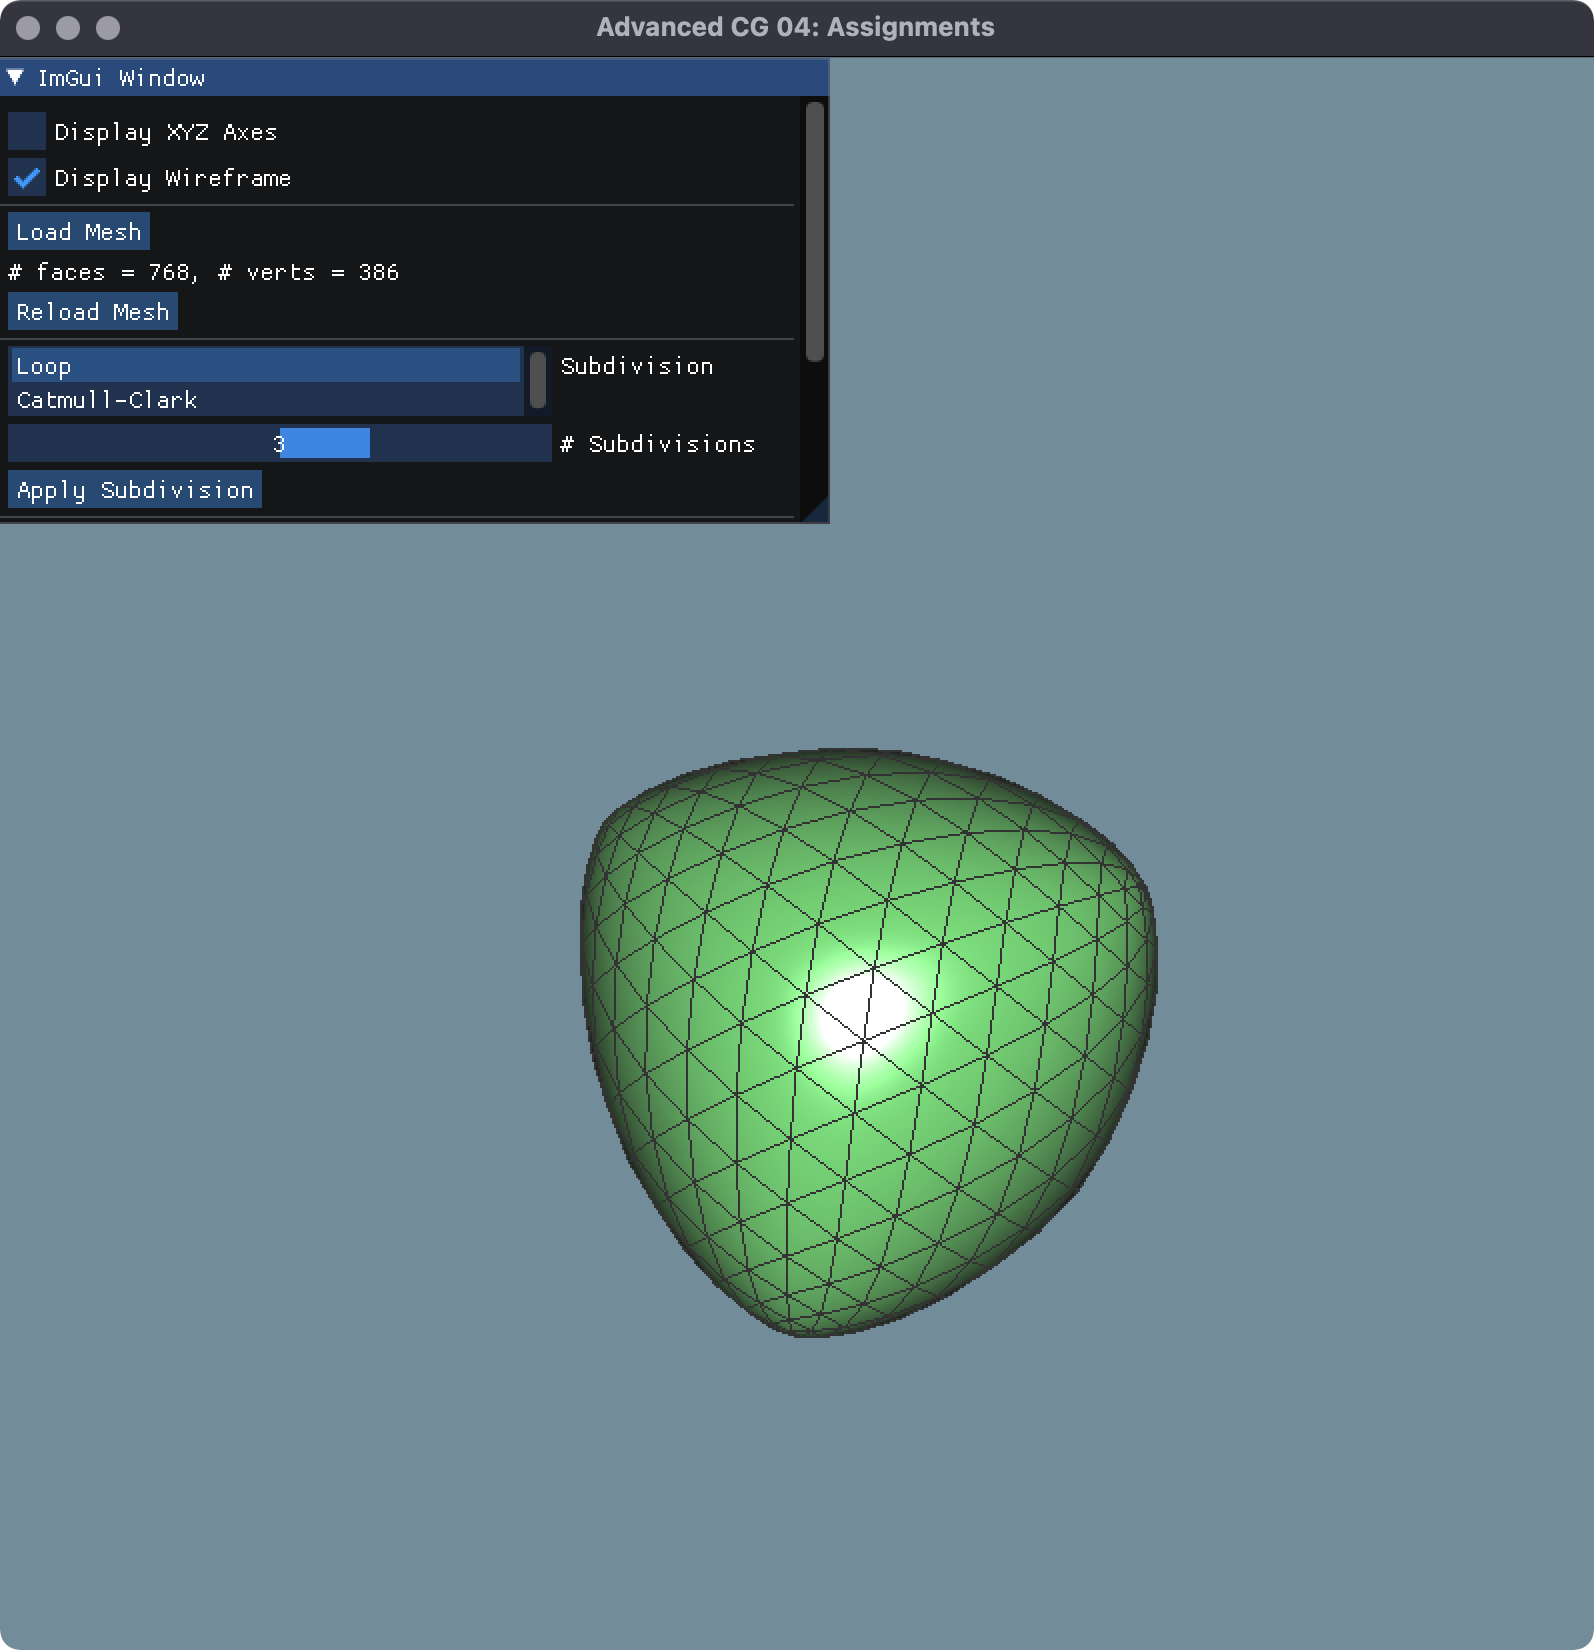
\includegraphics[width=45mm]{img/loop-cube-3.png}
      \caption{適用回数:3回}
    \end{center}
  \end{minipage}
\end{figure}

\begin{figure}[htbp]
  \begin{minipage}{0.33\hsize}
    \begin{center}
      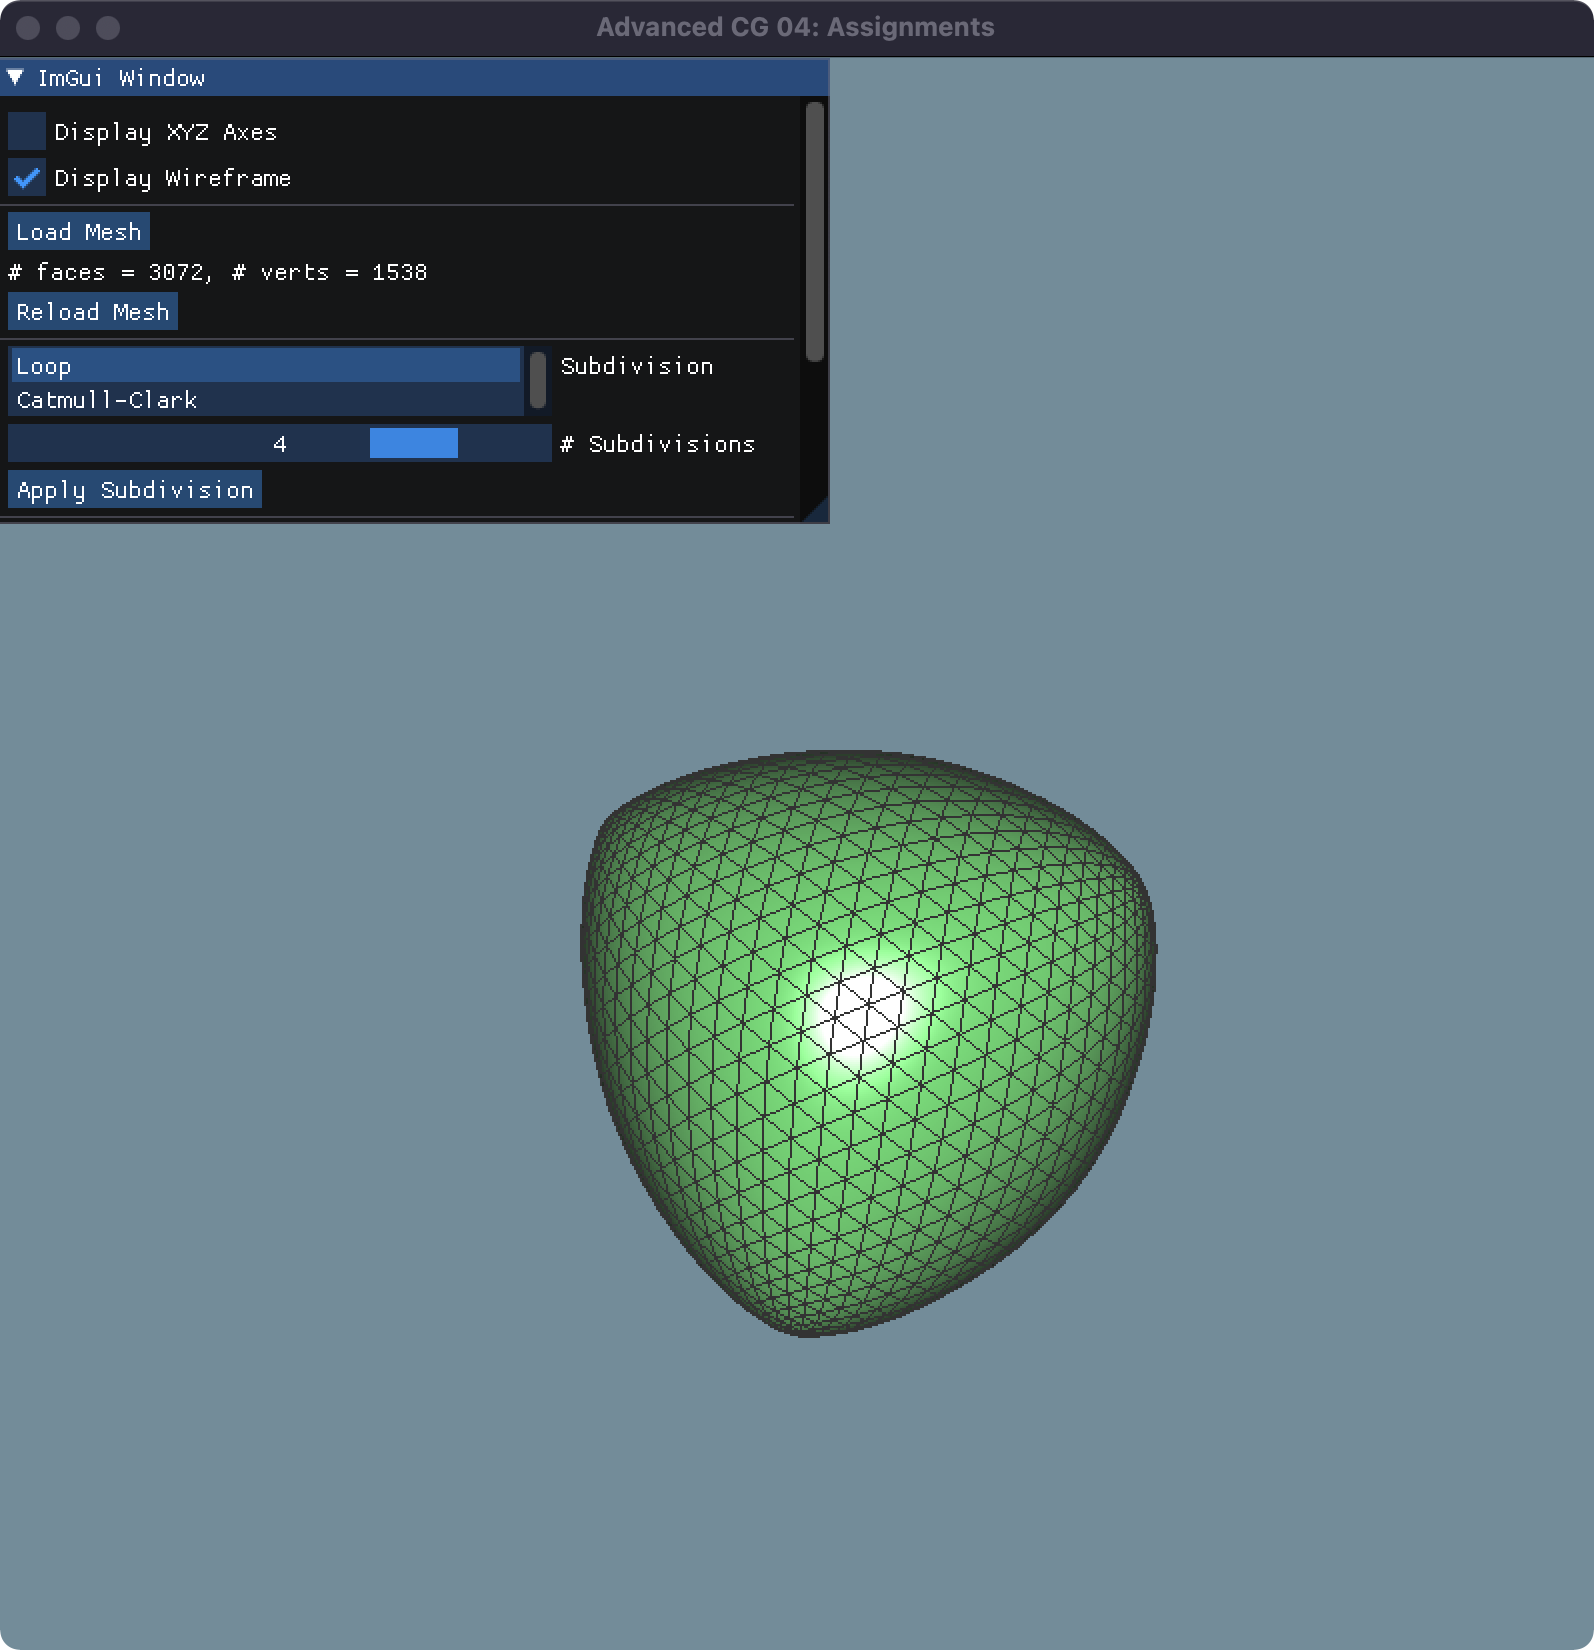
\includegraphics[width=45mm]{img/loop-cube-4.png}
      \caption{適用回数:4回}
    \end{center}
  \end{minipage}
  \begin{minipage}{0.33\hsize}
    \begin{center}
      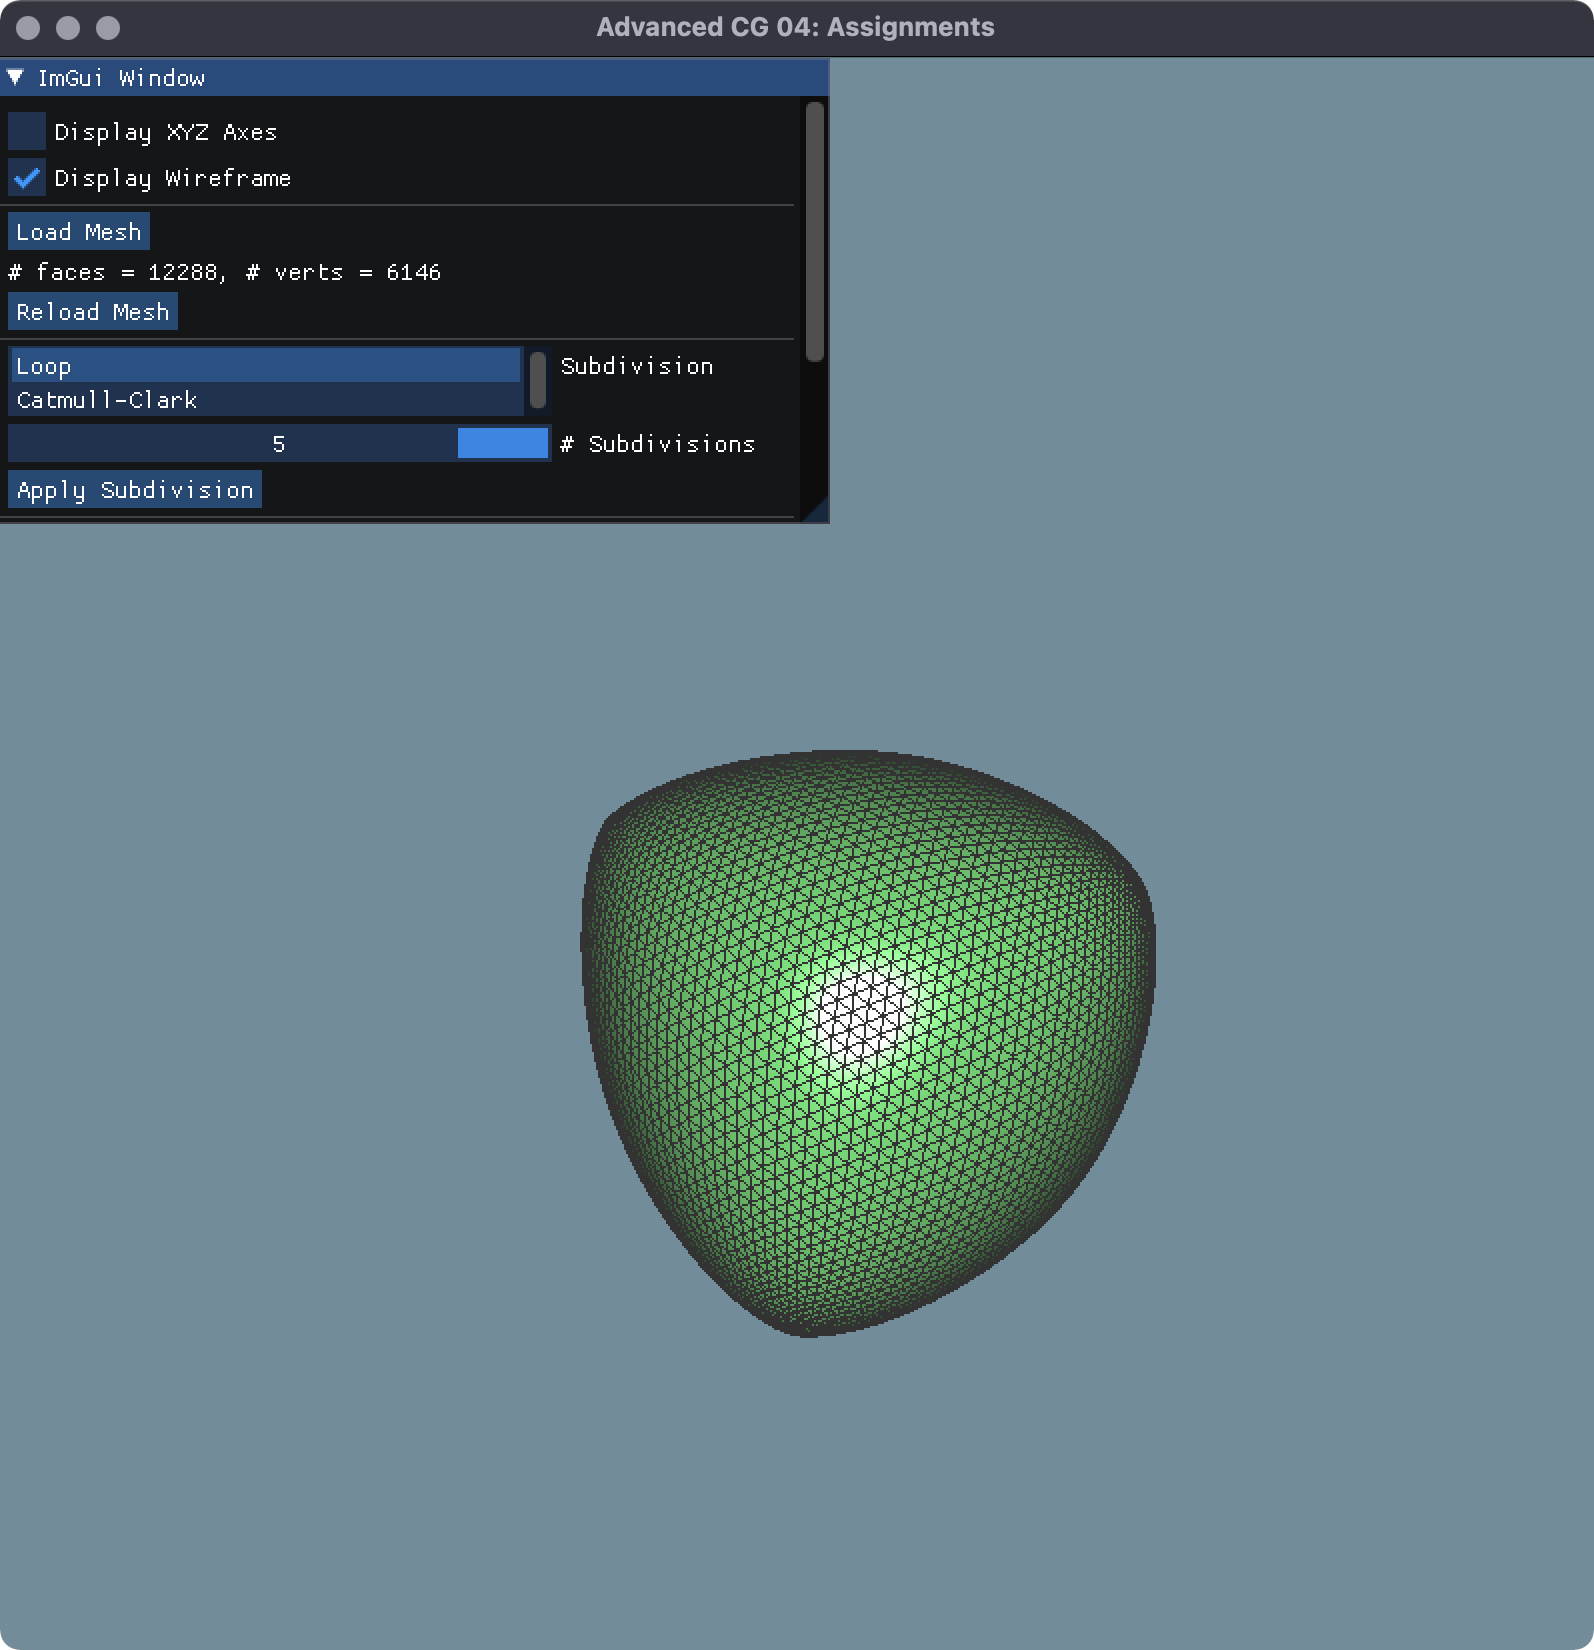
\includegraphics[width=45mm]{img/loop-cube-5.png}
      \caption{適用回数:5回}
    \end{center}
  \end{minipage}
\end{figure}

\subsubsection{Catmull-Clark細分割}
Catmull-Clark細分割をcube.objに対して実行した結果は以下のようになった。
\begin{figure}[htbp]
  \begin{minipage}{0.33\hsize}
    \begin{center}
      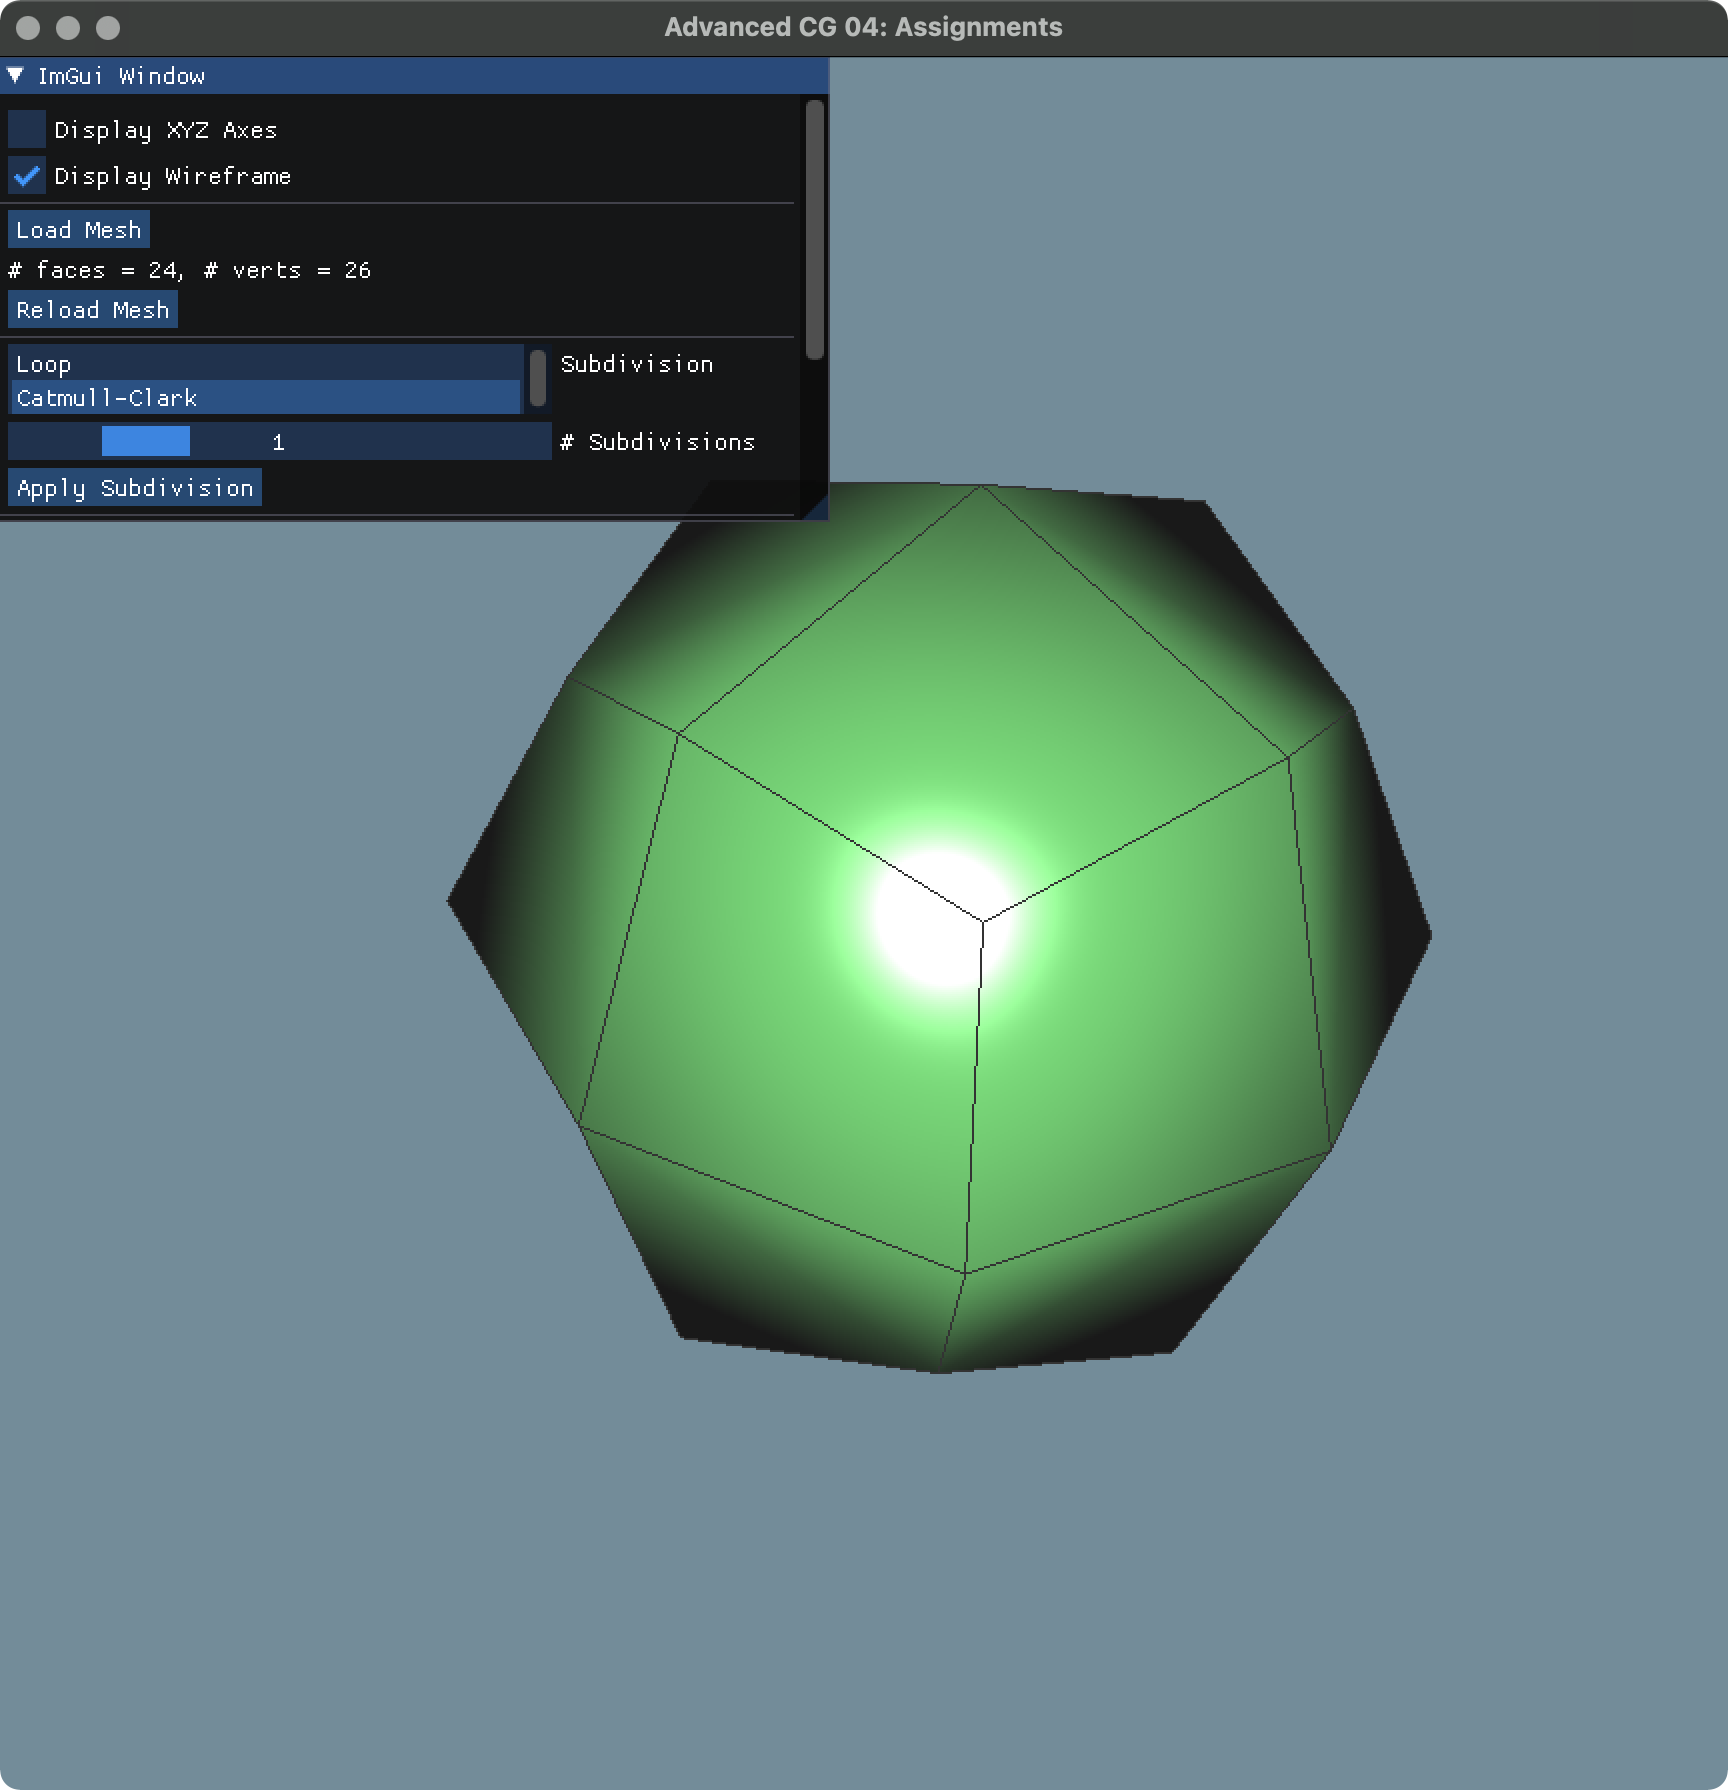
\includegraphics[width=45mm]{img/catmull-cube-1.png}
      \caption{適用回数:1回}
    \end{center}
  \end{minipage}
  \begin{minipage}{0.33\hsize}
    \begin{center}
      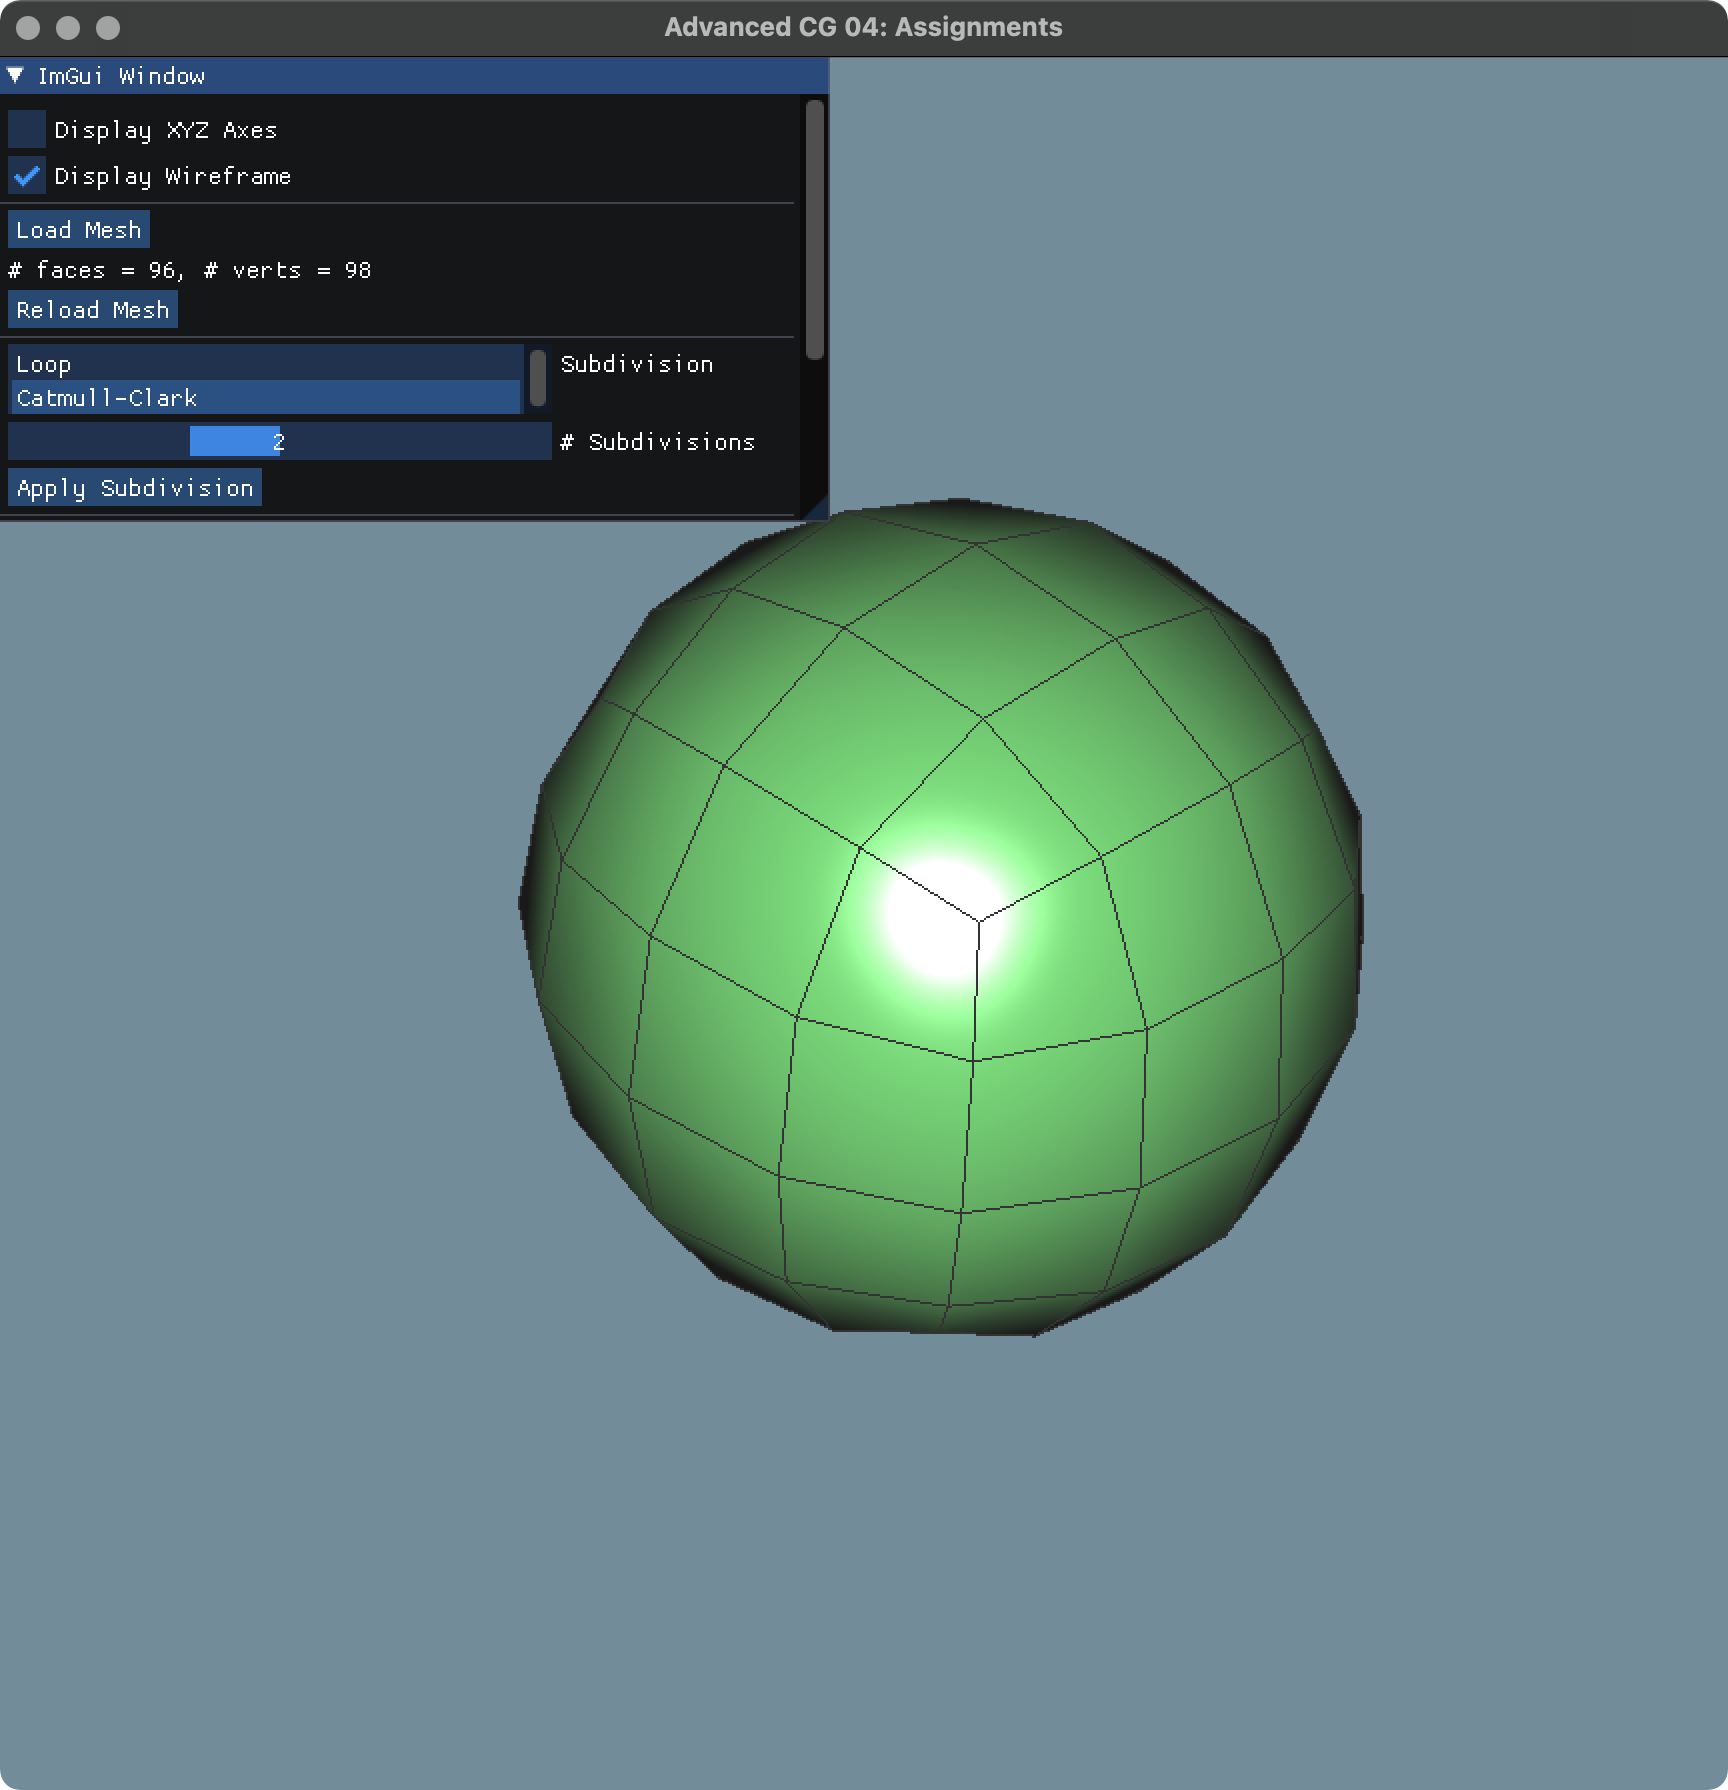
\includegraphics[width=45mm]{img/catmull-cube-2.png}
      \caption{適用回数:2回}
    \end{center}
  \end{minipage}
  \begin{minipage}{0.33\hsize}
    \begin{center}
      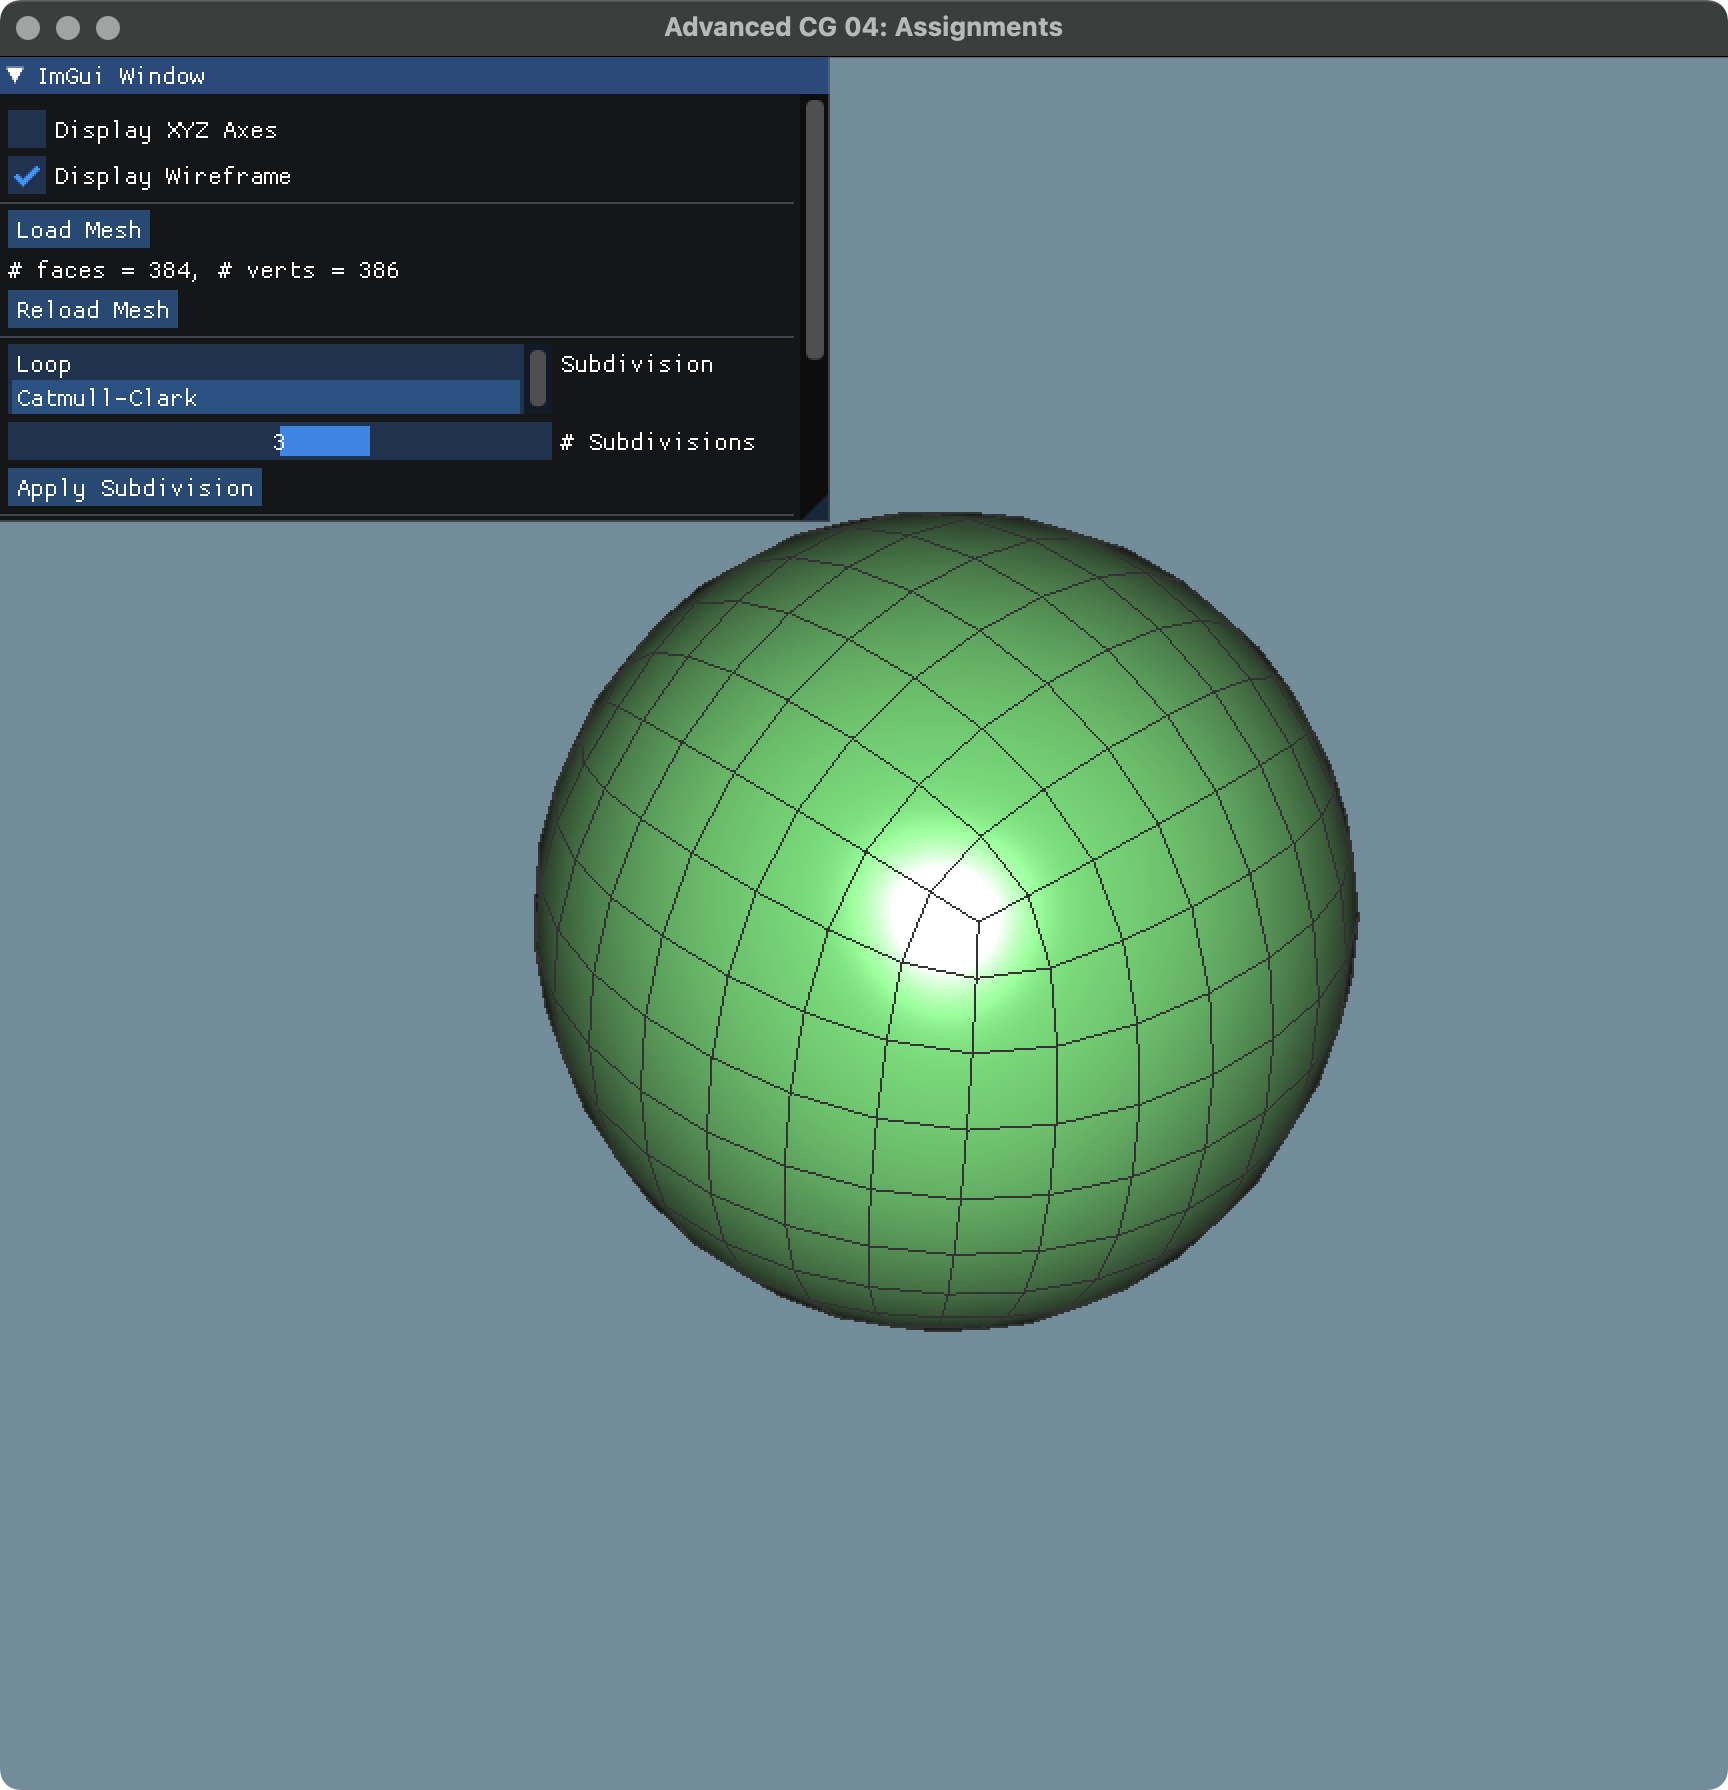
\includegraphics[width=45mm]{img/catmull-cube-3.png}
      \caption{適用回数:3回}
    \end{center}
  \end{minipage}
\end{figure}

\begin{figure}[htbp]
  \begin{minipage}{0.33\hsize}
    \begin{center}
      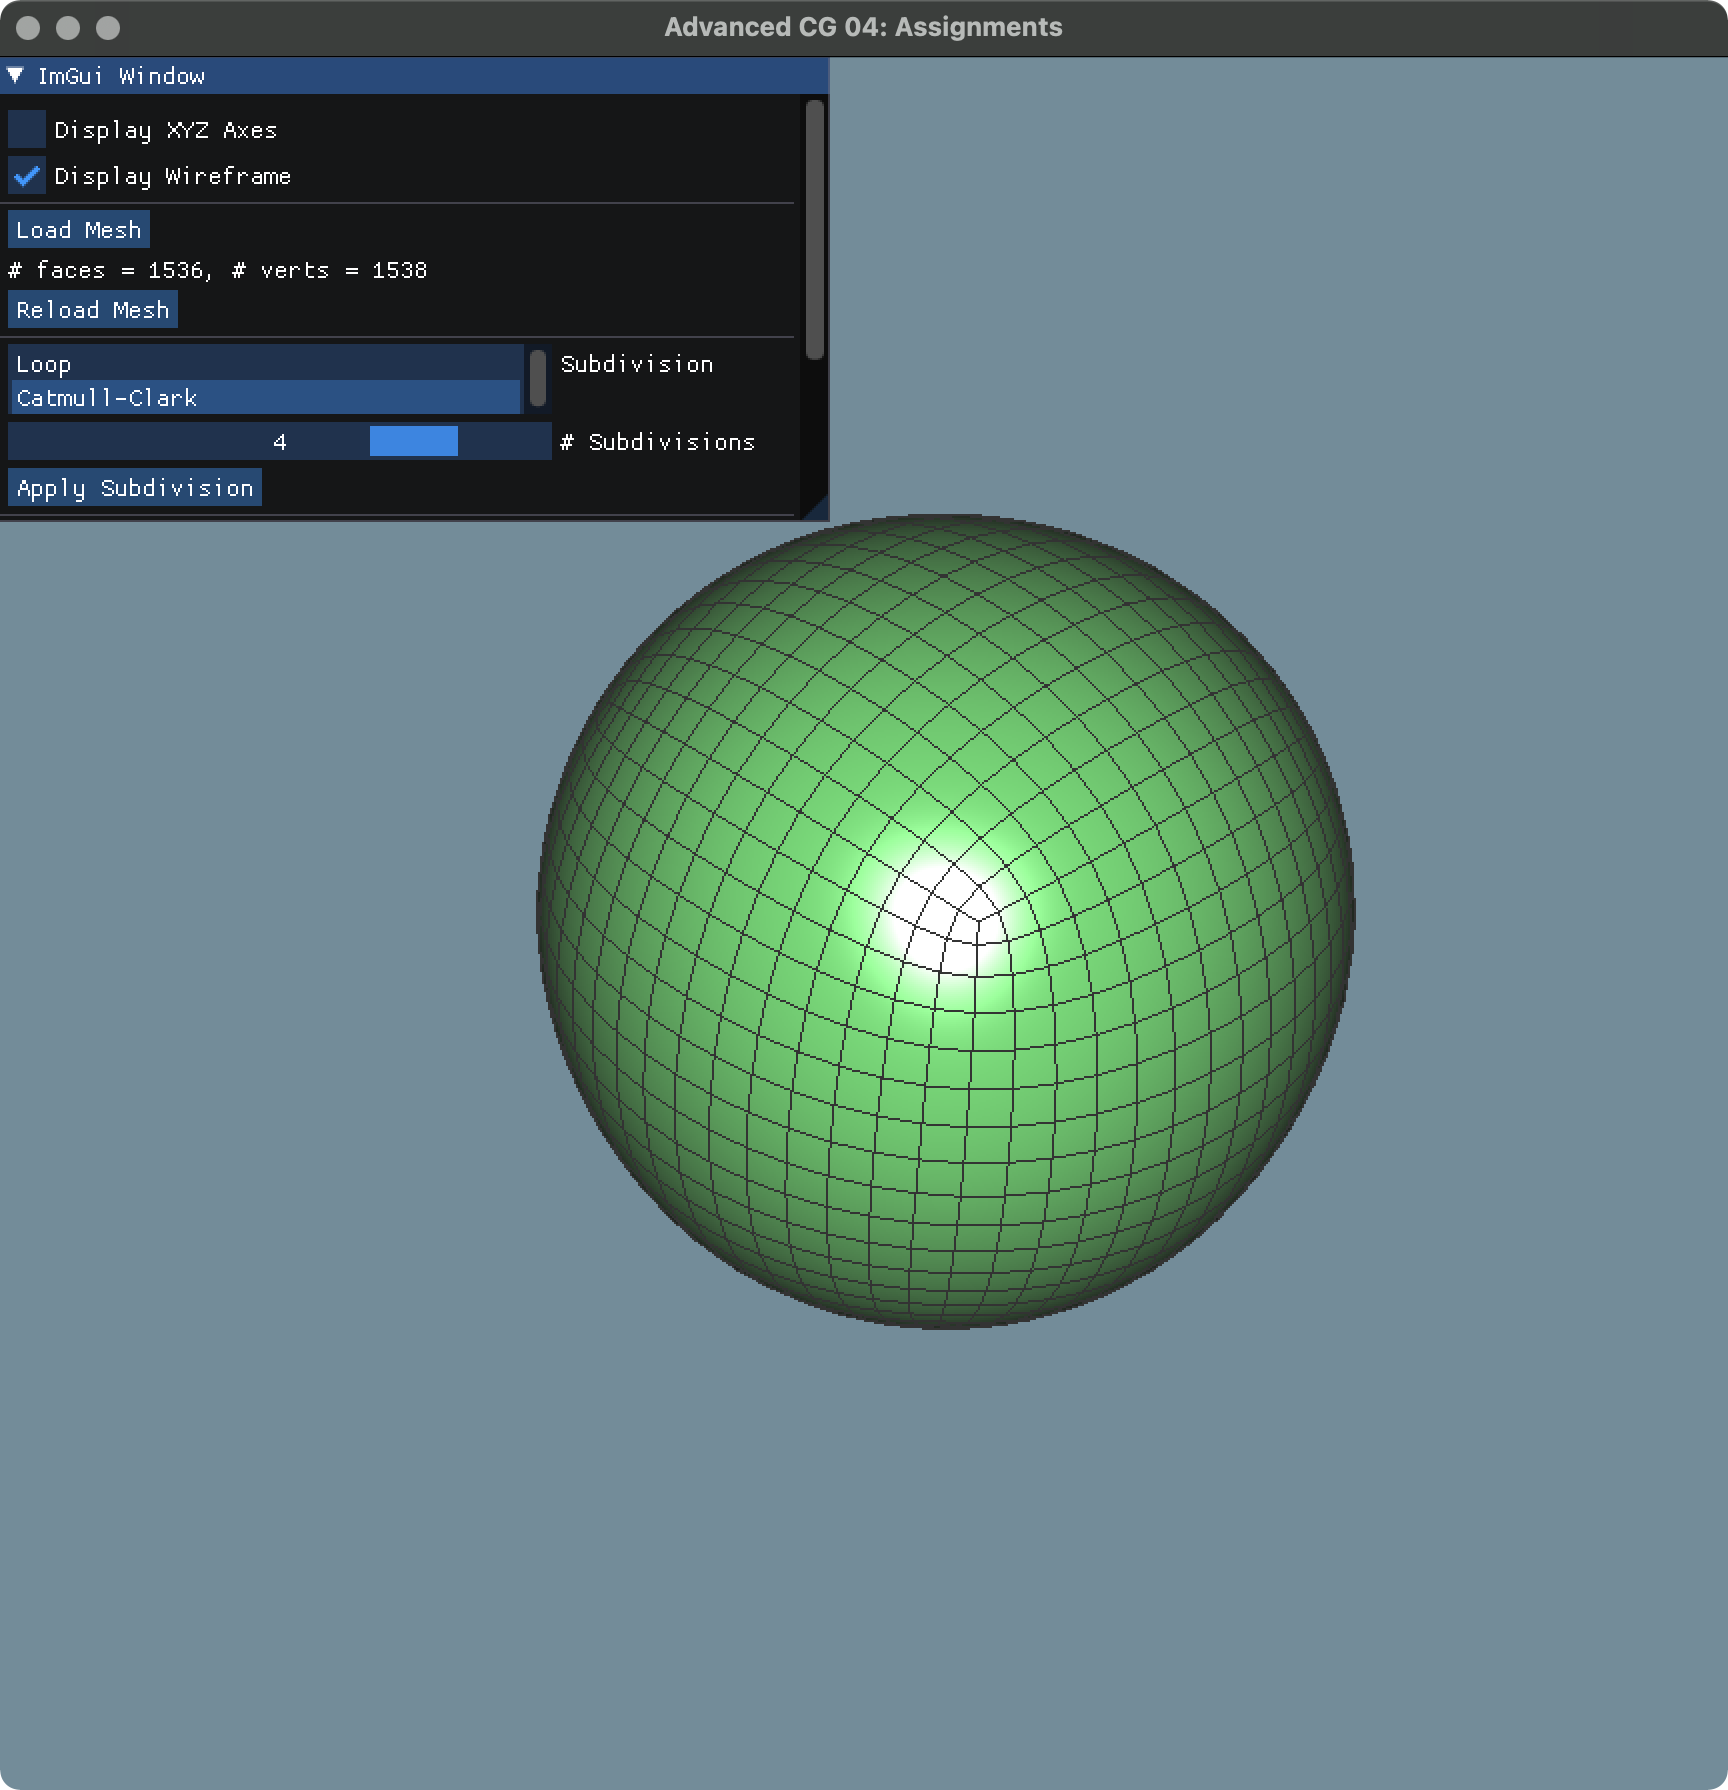
\includegraphics[width=45mm]{img/catmull-cube-4.png}
      \caption{適用回数:4回}
    \end{center}
  \end{minipage}
  \begin{minipage}{0.33\hsize}
    \begin{center}
      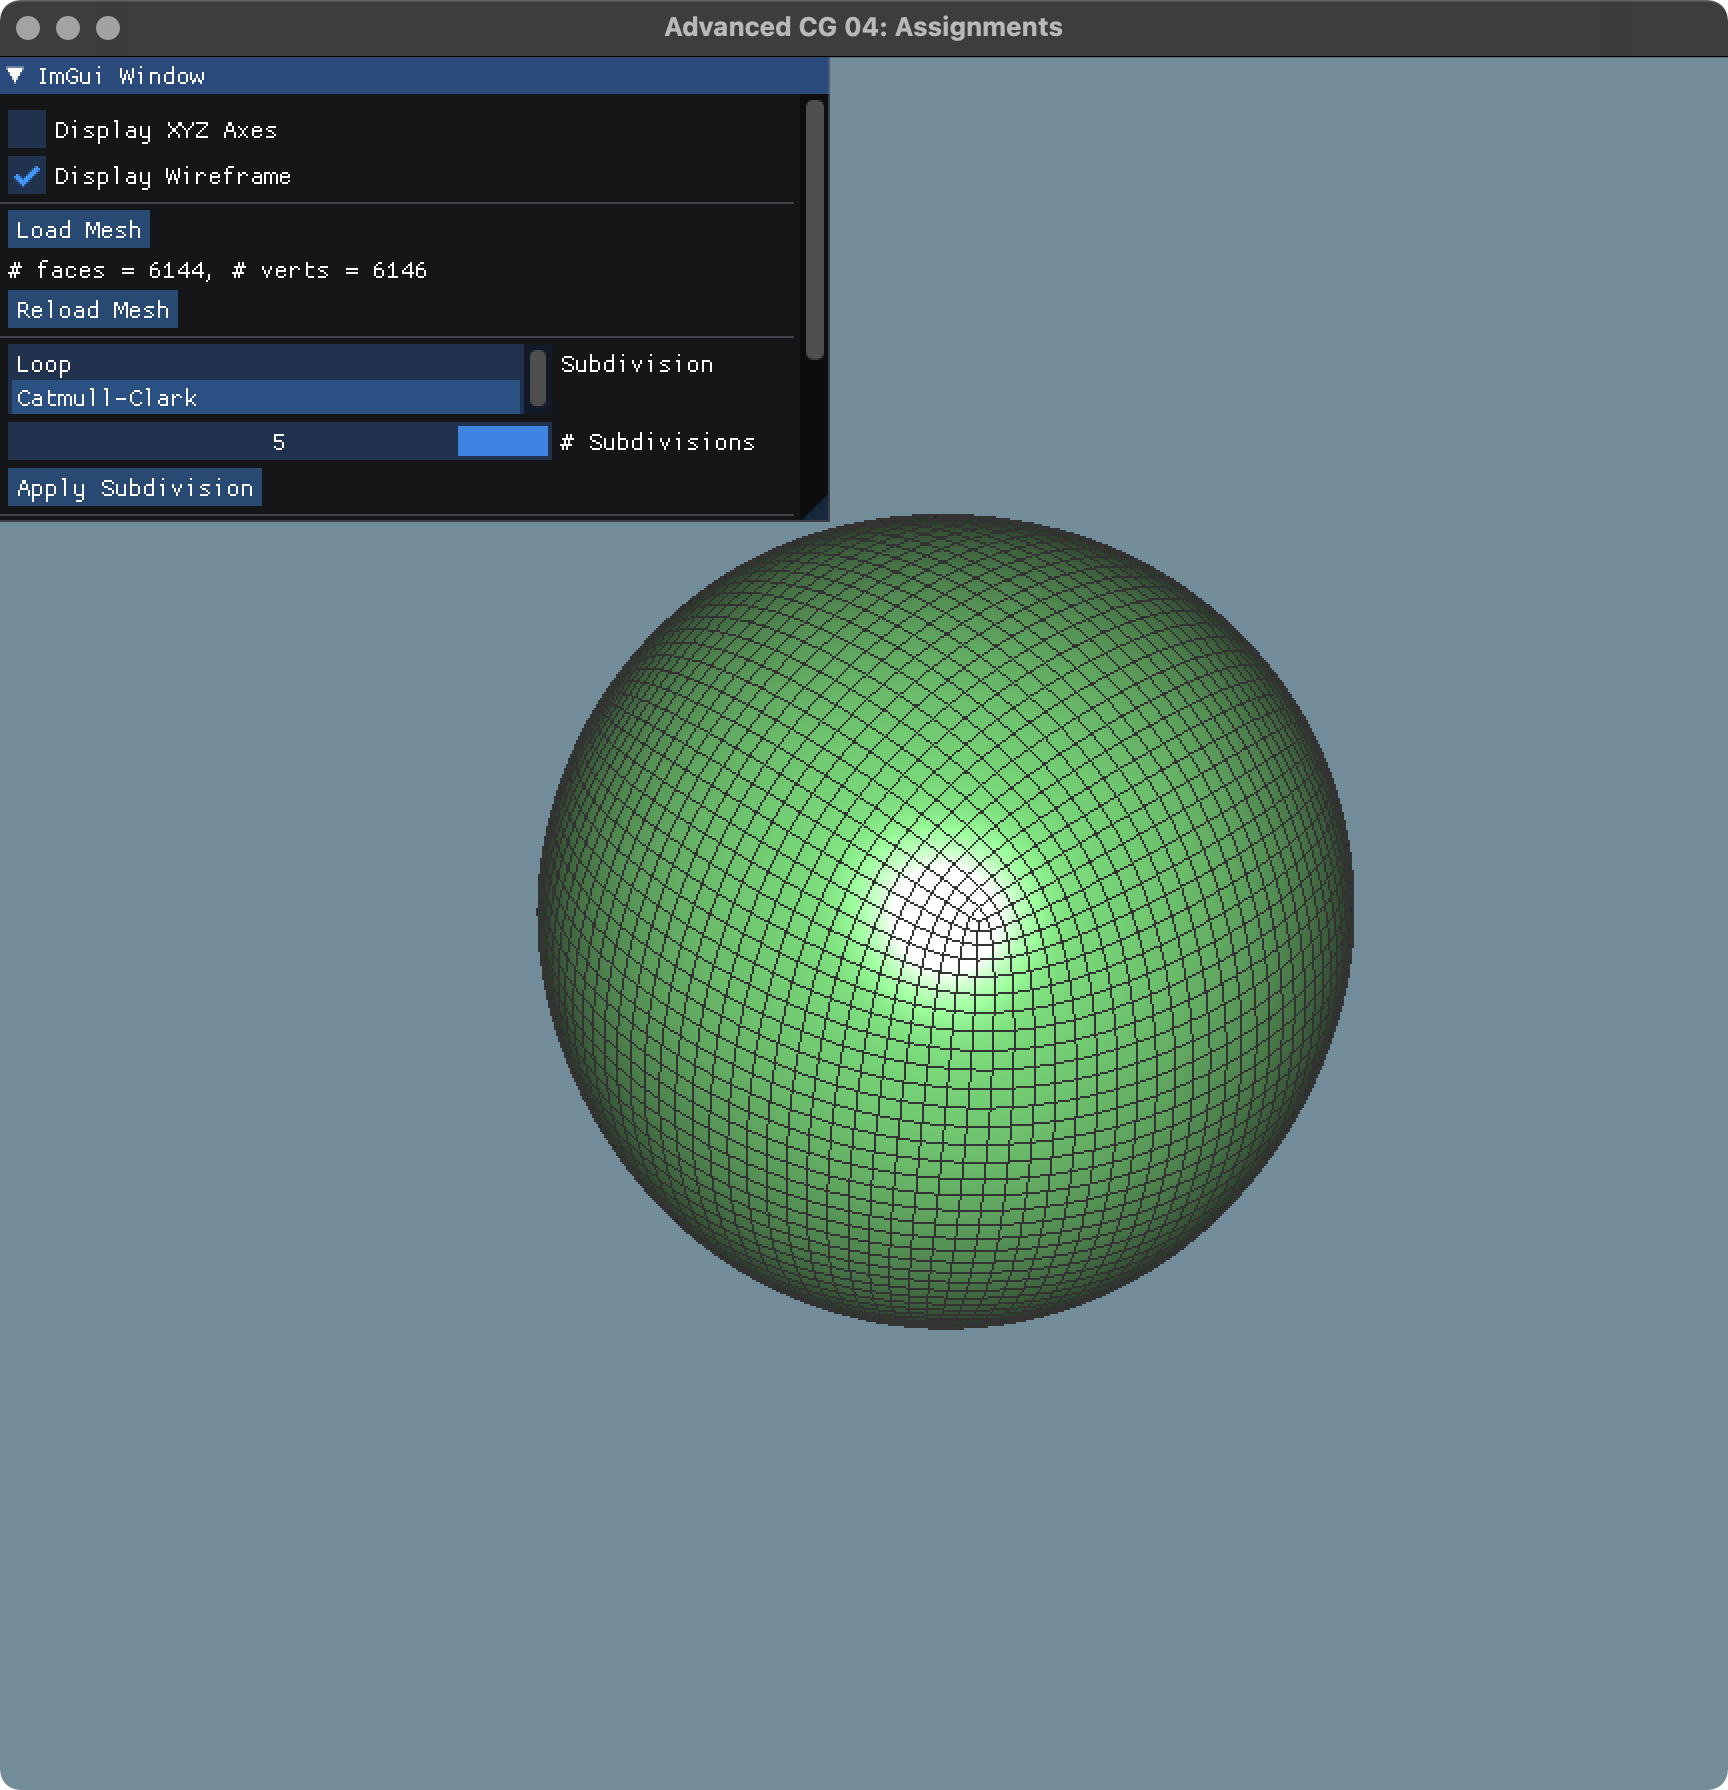
\includegraphics[width=45mm]{img/catmull-cube-5.png}
      \caption{適用回数:5回}
    \end{center}
  \end{minipage}
\end{figure}

\end{document}